\documentclass[a4paper,10pt]{article}
\usepackage{amsmath,amssymb,graphicx,float,subfig}

%defines
\def\bR{{\bf R}}
\def\bA{{\bf A}}
\def\bB{{\bf B}}
\def\bX{{\bf X}}
\def\bH{{\bf H}}
\def\bE{{\bf E}}
\def\bI{{\bf I}}
\def\bG{{\bf G}}
\def\bV{{\bf V}}
\def\bQ{{\bf Q}}
\def\btQ{{\bf \tilde Q}}
\def\bC{{\bf C}}
\def\btA{{\bf \tilde A}}
\def\b1{{\bf 1}}
\def\bx{{\bf x}}
\def\bb{{\bf b}}
\def\be{{\bf e}}
\def\bw{{\bf w}}
\def\by{{\bf y}}
\def\bz{{\bf z}}
\def\btx{{\bf{\tilde x}}}
\def\blambda{{\boldsymbol \lambda}}
\def\bgamma{{\boldsymbol \gamma}}
\def\btheta{{\boldsymbol \theta}}
\def\bbeta{{\boldsymbol \beta}}
\def\bnu{{\boldsymbol \nu}}
\def\bmu{{\boldsymbol \mu}}
\def\sigmaeps{{\sigma_{\epsilon}}}
\def\bxmode{{\hat \bx^{(0)}}}
\def\txmode{{\tilde \bx_{\mathrm{mode}}}}
\def\txsample{{\tilde \bx_{\mathrm{sample}}}}
\newcommand{\norm}[1]{\left\lVert#1\right\rVert}
\newcommand{\abs}[1]{|#1|}
%opening
\title{Minium Fuel Optimal Control}
\author{Santhosh Nadig}

\begin{document}

\maketitle
We have a linear dynamical system with states $x(t) \in \bR^n$ , $t = 0,1,\dots,N-1$, and actuator signal $u(t) \in \bR$. The dynamics of the system is given by the recursion
\begin{align}
x(t+1) = Ax(t) + b u(t)
\label{eq:rec}
\end{align}
where $A \in \bR^{n\times n}$ and $b \in \bR^n$ are given. We assume $x(0) = 0$. We need to choose the inputs $u(0),\dots,u(N-1)$ so as to minimize the total fuel consumed, which is given by
\begin{align}
F = \sum_{i = 0}^{N-1} f(u(t))
\label{eq:costfunc}
\end{align}
subject to the constraint that $x(N) = x_{\text{des}}$, where $N$ is the desired time horizon and $x_{\text{des}}$ is the desired final state. The function $f: \bR \rightarrow \bR$ is the fuel use map which gives the fuel usage as a function of the actuator input and is given by
\begin{align}
f = \begin{cases}
\abs{a} & \abs{a} \le 1 \\
2\abs{a} - 1 & \abs{a} > 1
\end{cases}
\label{eq:funcf}
\end{align}

From the initial condition and the recursion in (\ref{eq:rec}), it follows that
\begin{align*}
x(1) &= bu(0) \\
x(2) &= Abu(0) + bu(1) \\
x(3) &= A^2bu(0) + Abu(1) + bu(2) \\
\quad \vdots \\
x_{\text{des}} = x(N) &= A^{N-1}bu(0) + \dots + b \\
&= \begin{bmatrix}
 A^{N-1}b & A^{N-2}b & \dots &b
\end{bmatrix}
u.
\end{align*}

To express the cost function as a {\em linear} cost function, we use the epigraph trick. Minimizing the function $f$ (in (\ref{eq:funcf})) is the same as minimizing a linear objective in $t$ given by
\begin{align*}
\text{minimize} & \qquad t \\
\text{subject~to} & \qquad a \le t \\
& \qquad -a \le t \\
& \qquad 2a-1 \le t \\
& \qquad-2a-1 \le t
\end{align*}

Thus, we may express the cost function (and the minimization problem) as:
\begin{align}
\text{minimize} & \qquad \mathbf{1}^T t \nonumber \\
\text{subject~to} & \qquad Hu = x_{\text{des}} \nonumber\\
& \qquad  u \preceq t \nonumber \\
& \qquad  -u \preceq t \nonumber\\
& \qquad 2u-1 \preceq t \nonumber\\
& \qquad-2u-1\preceq t
\end{align}

For the example in A3.17 with the following data
\begin{align*}
A &= \begin{bmatrix}
-1 & 0.4 & 0.8 \\
1 & 0 & 0 \\
0 & 1 & 0
\end{bmatrix}, \qquad
b = \begin{bmatrix}
1 \\ 0 \\ 3
\end{bmatrix}, \qquad
x_{\text{des}} = \begin{bmatrix}
7 \\ 2 \\ -6
\end{bmatrix}, \qquad N = 30
\end{align*}
the optimal actuator input (solved both directly and as the above LP) is shown in the figure below.
\begin{figure}[ht]
\centering
  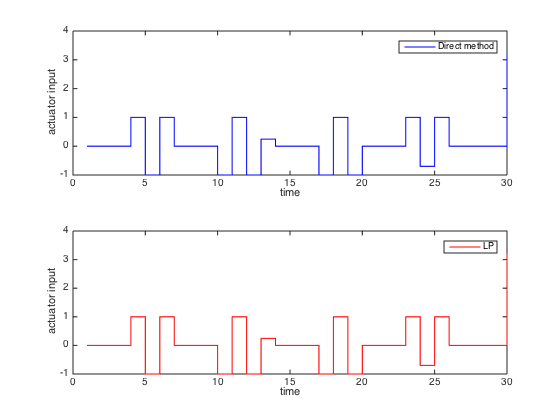
\includegraphics[width=9cm, height=9cm]{actuator_input.png}%
\end{figure}
\end{document}

